\chapter{Results}
In order to discern whether the choice of programming language has an environmental impact, we did experiments, each time changing a different aspect of the experiment to see if there is a significant difference between the performance of the languages. Most experiments used the programs to blur 78 high definition images.

\section{C++ and Python with OpenCV }
The first experiment we did was to simply run our programs with the chosen profiler of xctrace and cProfile to determine the runtime of each function of the program, blurring 78 images in total. We ran each benchmark 5 times and then calculated the average. The result of these experiments can be seen in graph x.

\begin{figure}[H]
	\centering
	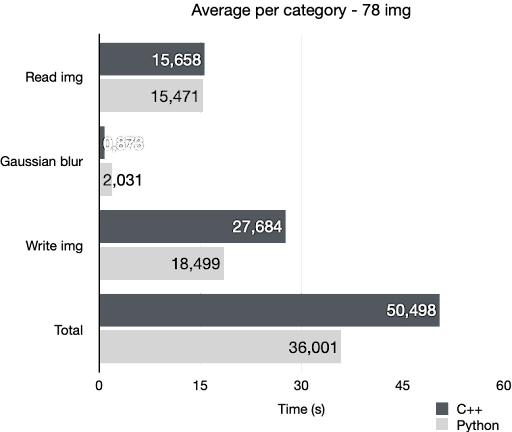
\includegraphics[scale=0.62]{average-78img.png}
	\caption{The average of 5 runs for each language}
	\label{figure:average-78img}
\end{figure}

These results were highly uncharacteristic. Based on previous research, we expected C++ to be faster than Python, not slower as seen in graph x. Most of the delay for C++ seems to come from writing the blurred image to the disk as seen in the write img bars in graph x.

\section{Saving to BMP instead of JPEG}
One approach to solving the significant delay of C++ when writing images to the disk, was to change the file type of the image for both languages. The default settings of the OpenCV package saved the image to whichever file type the image was originally; in our case that was JPEG (Joint Photographic Experts Group). By changing the file extension from JPEG to BMP (bitmap image file), the image file type would be changed on saving the image. Strangely, as seen in table x, this warped the data in such a way that reading the image now took longer for C++ and writing the image was quite a bit faster. We assume that this might be attributed to the library version but further research is needed to confirm this.

\begin{figure}[H]
	\centering
	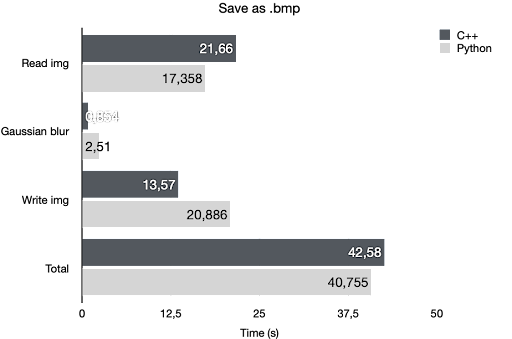
\includegraphics[scale=0.62]{bmp.png}
	\caption{Saving the image as a BMP file}
	\label{figure:bmp}
\end{figure}

\section{Using a script to benchmark}
The next experiment we did was to benchmark the programs using a script. A script is a sequence of instructions that are carried out subsequently by a computer, as seen in image x.

\begin{figure}[H]
	\centering
	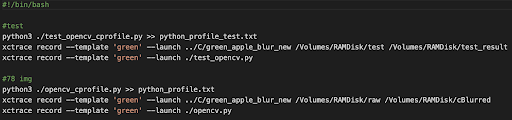
\includegraphics[scale=0.62]{script.png}
	\caption{The script used to profile the different programs}
	\label{figure:script}
\end{figure}

This was done in order to minimise the time between running each benchmark and therefore minimising the difference between computer operations. It also allowed us to randomise the different programs to see how one program running before or after another might affect its performance.

\begin{figure}[H]
	\centering
	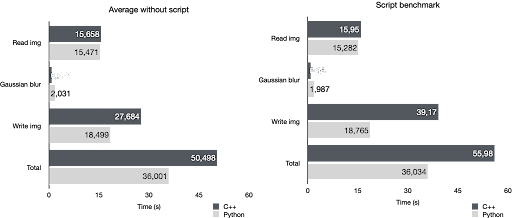
\includegraphics[scale=0.62]{script-vs-noscript.png}
	\caption{Comparing the results of a script versus no script}
	\label{figure:script-vs-noscript}
\end{figure}

We can seen in chart x, when compared to chart y, that there is a small difference between the readings when using a script. This is shown especially when writing the image in C++. This might be attributed to the system load caused by running all programs so quickly after each other.

\begin{figure}[H]
	\centering
	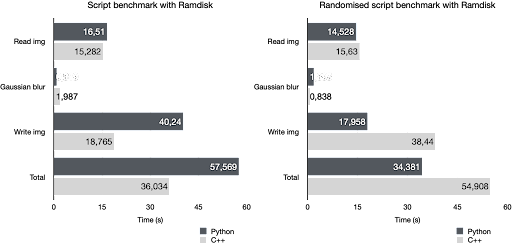
\includegraphics[scale=0.62]{two-scripts.png}
	\caption{Comparing two different scripts}
	\label{figure:two-scripts}
\end{figure}

Graphs x and y show two benchmarks with a different order of the script, both using a RAMdisk. Each was measured by blurring 78 images. There is a slight difference between the two benchmarks, the randomised one running about two seconds faster. Overall, the proportions of the different benchmarks stayed the same.

\section{RAMdisk}
A RAMdisk is a block of random-access memory that a computer's software is treating as if the memory were a disk drive. It can be used to accelerate the reading and writing of files. We installed a RAMdisk using the command “diskutil erasevolume HFS+ "RAMDisk" `hdiutil attach -nomount ram://2097152`” in the terminal. This creates a RAMdisk with 1 GB of storage space.

\begin{figure}[H]
	\centering
	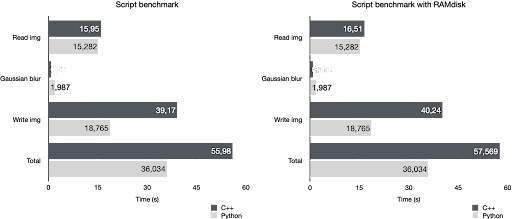
\includegraphics[scale=0.62]{ramdisk.png}
	\caption{Comparing benchmarks without and with the use of a RAMdisk using the same script}
	\label{figure:ramdisk}
\end{figure}

Compared to the benchmarks with no RAMdisk, running the scripted benchmarks with a RAMdisk surprisingly returns a decreased performance. However, the difference is so slight that it is not confirmed whether this is due to the RAMdisk or another influence.

\section{Running the programs on a different computer}
In order to find out whether the disk I/O was influenced by the computer hardware we decided to test the programs on a different computer. We utilised the same computer type in a different configuration: the MacBook Pro from 2021 with an M1 Pro Apple Silicon CPU, 32 GB of RAM and a 1 TB SSD. To run the programs on this new configuration we had to install Python version 3.10.3 instead of the previously used 3.8.12. Our software was not compatible with the new M1 chip so it had to be recompiled for Apple Silicon.

\begin{figure}[H]
	\centering
	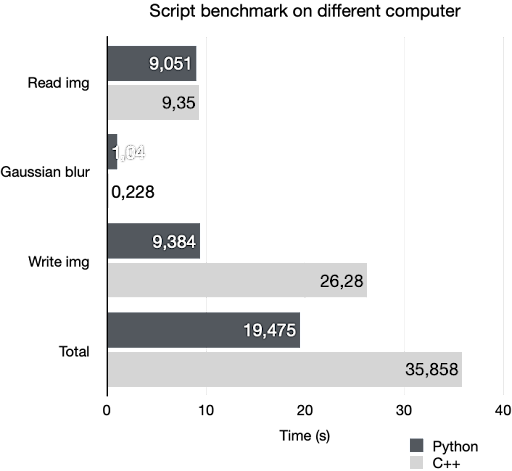
\includegraphics[scale=0.62]{different-comp.png}
	\caption{Script benchmark on a different computer}
	\label{figure:different-comp}
\end{figure}

Graph x shows a similar distribution of runtime for the benchmark but an overall acceleration of 15 to 20 seconds as compared to the other computer. The results are as expected since this computer is a newer model and has more powerful hardware.

\section{Profiling C++ and Python on Linux}
In order to rule out the possibility of the operating system influencing the unexpectedly slow C++ runtime, we decided to experiment with our programs on a different operating system. Using a virtual machine, we created an Ubuntu Linux instance to benchmark our programs. This required some adjusting as the executable made for macOS was not compatible with Linux and Linux obviously does not support the macOS instruments profiler. We compiled the C++ code with the cmake tool to create the new executable. As a profiler, we used the GCC (GNU Compiler Collection) compiler native fprofile command. For Python, it was still possible to use the cProfile profiler. We ran each program five times and calculated the average as seen in graph x.

\begin{figure}[H]
	\centering
	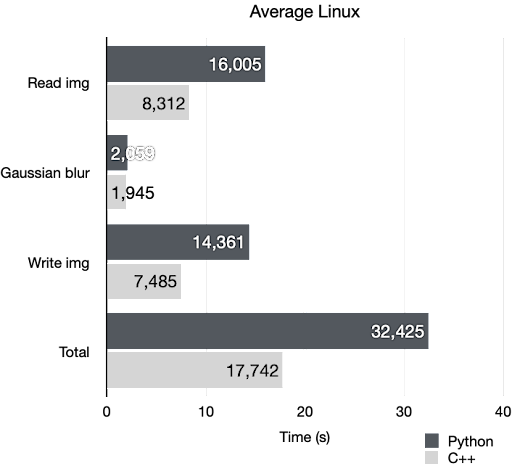
\includegraphics[scale=0.62]{linux.png}
	\caption{The average for the programs run on Linux}
	\label{figure:linux}
\end{figure}

Interestingly, on Linux, the C++ program performed a lot faster than Python; 14,683 seconds faster to be exact. This might once again be attributed to OpenCV being optimised in a different way for a different operating system and therefore performing better on Linux.

\section{C++ using OpenCV from VCPKG}
One theory we had for the delay of C++ for disk output was that it was due to how the OpenCV library function handled writing to the disk. After doing some further research, we found that the standard OpenCV package for Python is a different version from what is standard for C++. Using VCPKG, a C/C++ dependency manager \cite{vcpkg}, we were able to download the same version as used for Python and use it with C++. Benchmarking the programs with 100 randomly generated images shows the results in graph x. Now, we can see only a very insignificant difference between the two programming languages, as compared to before.

\begin{figure}[H]
	\centering
	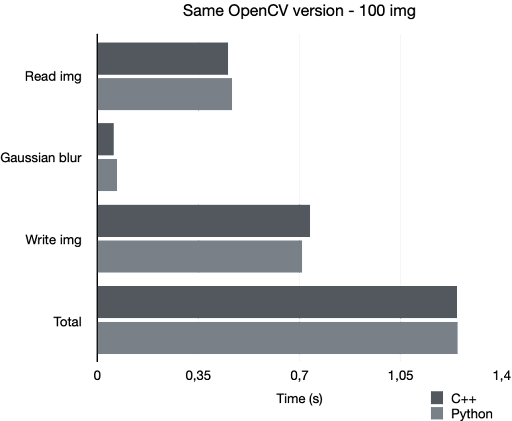
\includegraphics[scale=0.62]{same-opencv.png}
	\caption{Average of results using the same OpenCV version}
	\label{figure:same-opencv}
\end{figure}

We can see that the total runtime is significantly less than when using the previous images. This can probably be attributed to the randomly generated images, which seem to have a lower resolution and are therefore faster to be processed. However, this is not important for this study as only the comparison of C++ and Python is of any consequence and not the overall performance for both.

\section{The error interval}
An error interval is a property of the instrument and the user, and will remain the same for all readings taken, provided the scale is linear \cite{errorinterval}. It can be determined by finding the fraction of the smallest readable division on the instrument. In the case displayed in table x, benchmarking Python has yielded the error intervals in the last row, which is the same for each reading, as it is using the same instrument.

\begin{figure}[H]
	\centering
	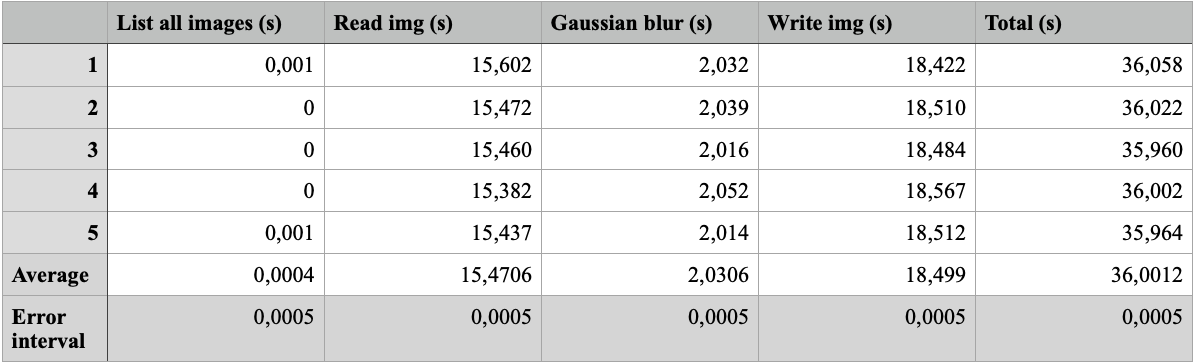
\includegraphics[scale=0.62]{error-interval.png}
	\caption{Python profiler average with error interval}
	\label{figure:error-interval}
\end{figure}

From this we can determine that if we have a reading of e.g. 18,500, with error interval it is actually between 18,4995 and 18,5005. Whilst this allows us to have a realistic interpretation of our measurements, it also does not affect our observations since all proportions are still the same.

\section{Energy consumption}
To confirm that runtime was congruous with energy consumption, we used the Intel Power Gadget to approximately measure the energy consumption of each program, both using the standard form of OpenCV with no RAMdisk. In the experiment, C++ had a runtime of 58,233 seconds, and Python had a runtime of 38,889 seconds.

\begin{figure}[H]
	\centering
	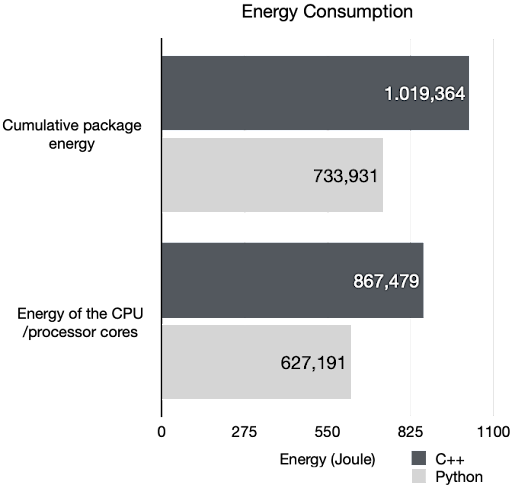
\includegraphics[scale=0.50]{energy-consumption.png}
	\caption{Energy consumption of the programs in Joule}
	\label{figure:energy-consumption}
\end{figure}

We can see in graph x that the proportion of runtime to energy consumption is approximately the same. C++ used more energy than Python for the same program. Python’s runtime is 66,78\% of the C++ runtime, and Python’s energy consumption is 72,00\% of C++’s energy consumption overall and 72,30\% of the energy of the CPU/processor cores. These results indicate that runtime is an approximate indicator of energy consumption.
